\documentclass{article}
\usepackage[utf8]{inputenc}

% Language setting
% Replace `english' with e.g. `spanish' to change the document language
\usepackage[english,russian]{babel}
\usepackage{amsmath}

%графика
\usepackage{wrapfig}
\usepackage{graphicx}
\usepackage{pgfplots}
\usepackage{tikz}


\usepackage{tcolorbox}

% Set page size and margins
% Replace `letterpaper' with `a4paper' for UK/EU standard size
\usepackage[letterpaper,top=2cm,bottom=2cm,left=3cm,right=3cm,marginparwidth=1.75cm]{geometry}

% Useful packages
\usepackage{amsmath}
\usepackage{amssymb}
\usepackage{graphicx}
\usepackage{fixltx2e}
\usepackage[colorlinks=true, allcolors=blue]{hyperref}

\usepackage{geometry}
\geometry{left=25mm,right=25mm,
 top=25mm,bottom=25mm}


\title{Quantitative Analytics.\\
Lectures. Week 3. \\
Options Trading Strategies.\\
Стратегии торговли опционами.}
\author{Gorelov Vasiliy}

% Колонтитулы
\usepackage{fancyhdr}
\pagestyle{fancy}
\renewcommand{\headrulewidth}{0.1mm}  
\renewcommand{\footrulewidth}{0.1mm}
\lfoot{}
\rfoot{\thepage}
\cfoot{}
\rhead{CMF-2022}
\chead{}

\begin{document}
\maketitle

% Оглавление
\setcounter{tocdepth}{1} % {2} - в оглавлении участвуют chapter, section и subsection. {1} - только chapter и section
\renewcommand\contentsname{Contents}
\tableofcontents
\newpage

% \section{Dictionary, Definitions, Abbreviations}

% \subsection{Dictionary}
% \begin{itemize}
%     \item IR - Interest rate - процентная ставка.
%     \item Compounding - платежи (idk)
% \end{itemize}

% \subsection{Definitions and Abbreviations}
% \begin{itemize}
%     \item SAR - Stated annual rate.
%     \item EAR - Effective annual rate.
%     \item FoC - Frequency of Compounding
%     \item PMT - Payment
%     \item r - Interest rate (at the moment). 
% \end{itemize}

\renewcommand{\labelitemi}{\tiny$\bullet$}
\renewcommand{\figurename}{Fig.}

 \section{Стратегии covered call и protective put}
 \begin{itemize}
     \item \textbf{Protective put} - это метод управления инвестициями, предназначенный для защиты от падения стоимости акций. Он создается путем покупки акции и put опциона на эту акцию.
     \begin{figure}[h]
    \centering
    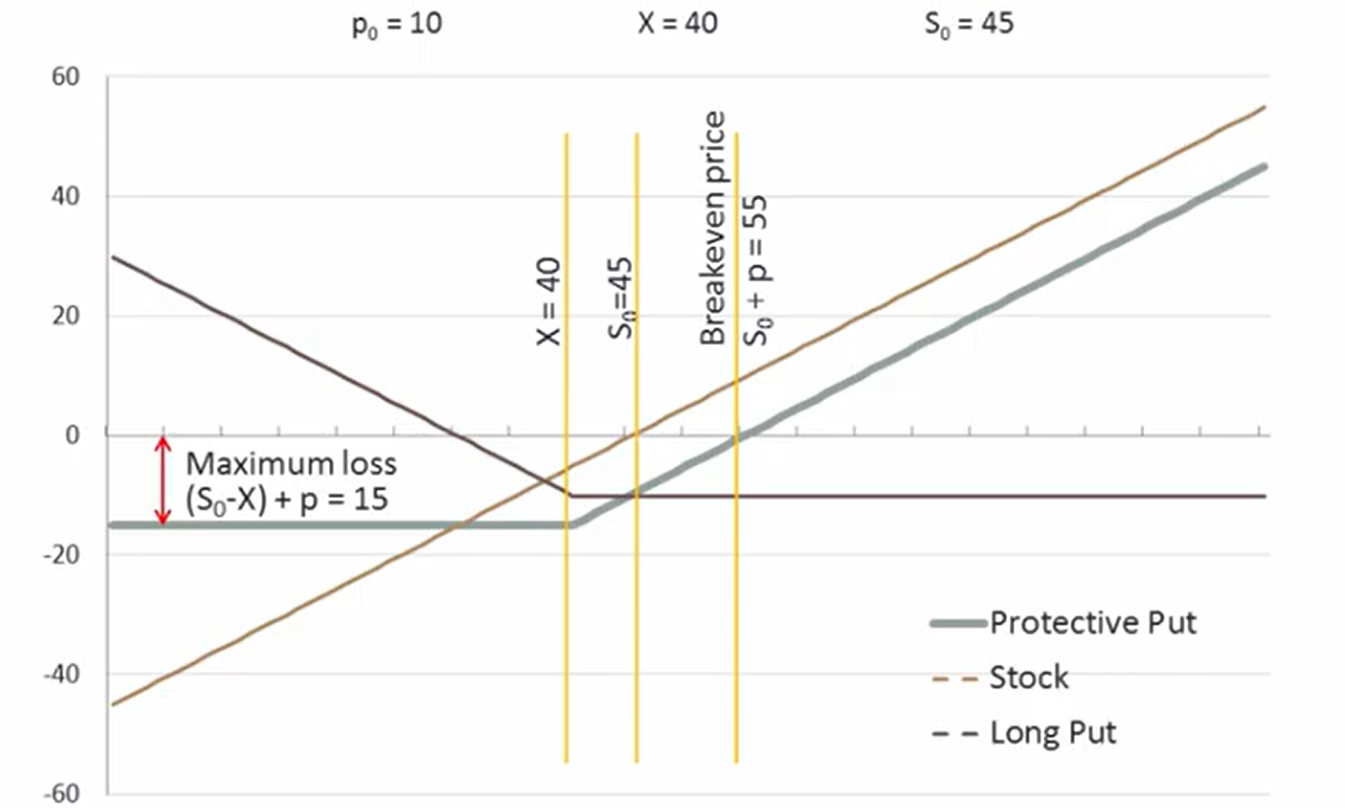
\includegraphics[width=0.7\textwidth]{protective put.png}
    \caption{Стратегия protective put}
    \label{Стратегия protective put}
    \end{figure}

     \item \textbf{Covered call} - это метод управления инвестициями, предназначенный для обмена потенциального роста акции на фиксированную премию. Он строится путем покупки акции и продажи call опциона на эту акцию.
     
     \begin{figure}[h]
     \centering
    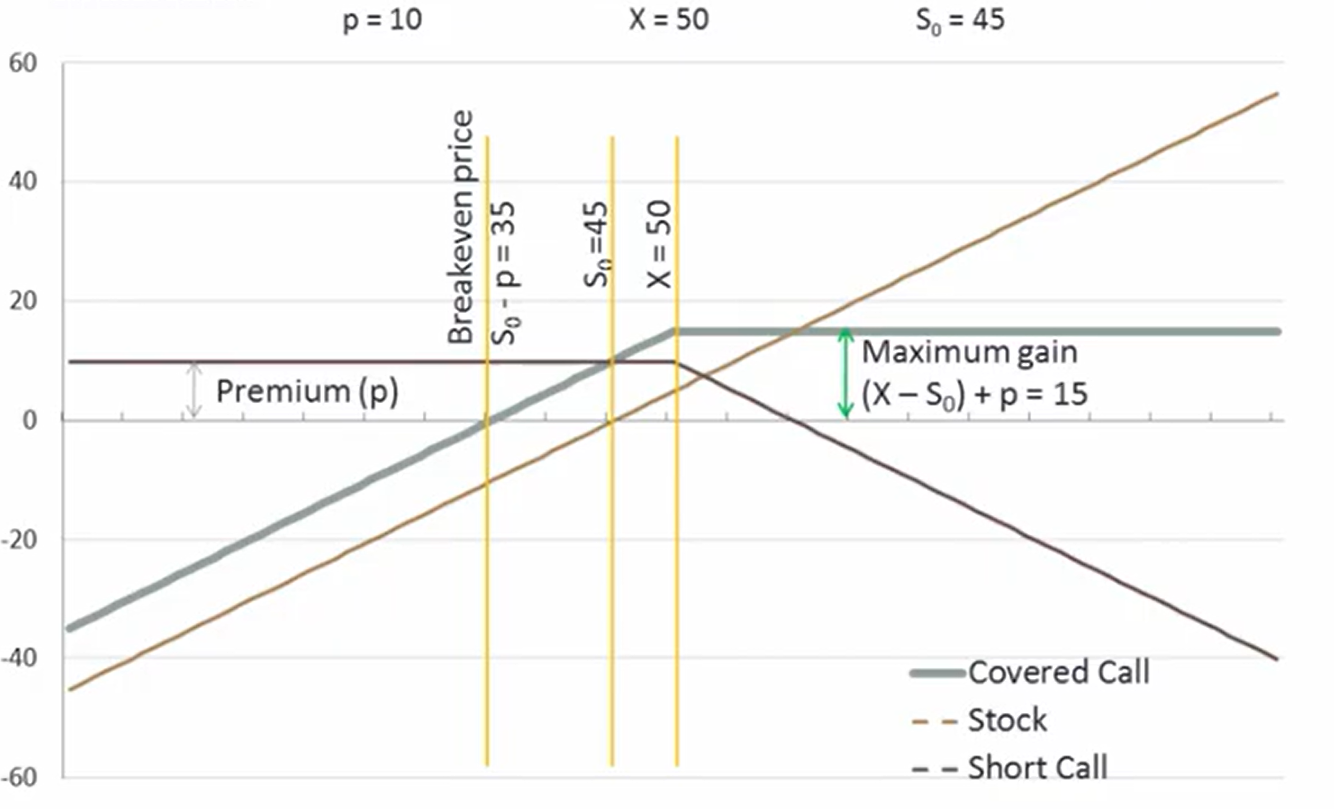
\includegraphics[width=0.7\textwidth]{covered call.png}
    \caption{Стратегия covered call}
    \label{Стратегия covered call}
    \end{figure}
     
 \end{itemize}
 
 \newpage
 \section{Инструменты с защитой капитала(principal protected note, PPN)}
 \textbf{Инструмент с защитой капитала(principal protected note, PPN)} - это финансовый инструмент состоящий из опциона так, чтобы инвестор получал прибыль от любого роста цены определённого портфеля без риска потерь.\\
 Предположим, что портфель A состоит из:
 \begin{itemize}
 \item Годовой безкупонной облигации, выплачивающей 1000\$ через год.
 
 \item Годового call опциона на индекс, который сейчас стоит 1000\$ со strike ценой 1000\$.
 
 \end{itemize}

  \raggedright Держатель портфеля A получит прибыль от роста цены индекса. И ничего не потеряет, если цена индекса пойдет вниз. Это свойство очень привлекательно для инвесторов, которые боятся риска.\\
 Полное исполнение PPN(т.е. держатель получает 100\% прибыли) возможен только для портфелей, которые приносят доход.
 Чтобы это заметить, глянем на это уравнение :\\
 \centering \textbf{p + S = c + PV(X)}\\
 \raggedright Из-за того, что сейчас опцион на индекс в деньгах(at the money), put-call parity дает, что:\\
 \centering \textbf{c = p + S - PV(S)}\\
 \raggedright Выражение выше подразумевает, что: \\
 \centering \textbf{c > S - PV(S)}\\
 \raggedright
 
 
 \section{Использование и выплата в различных spread стратегиях}
 
 
\begin{wrapfigure}{r}{0.4\textwidth}
    \centering    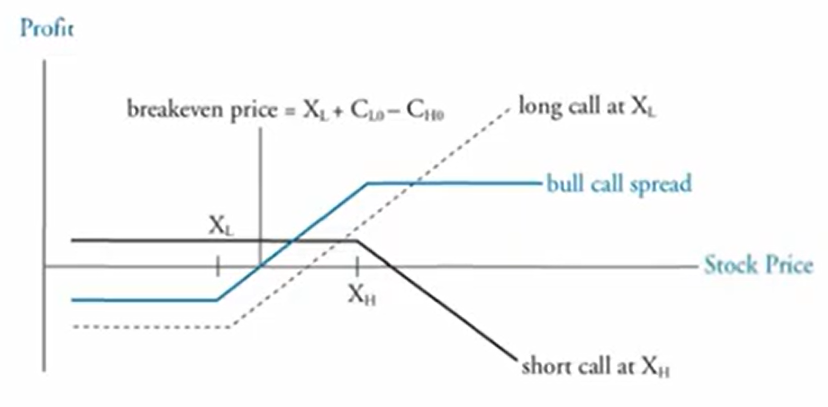
\includegraphics[width=0.4\textwidth]{bull call spread.png}
    \centering    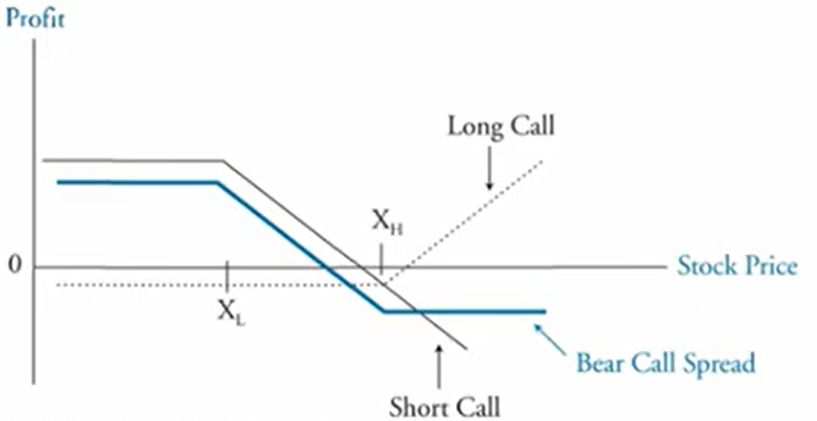
\includegraphics[width=0.4\textwidth]{bear call spread.png}
\end{wrapfigure}


 \textbf{Bull call spread:}
 \begin{itemize}
 \item Купить: call опцион с \textbf{меньшей} strike ценой.\\
Продать: call опцион с \textbf{большей} strike ценой.
\item Предположение: цена underlying актива вырастет.
\item Максимальная прибыль: $ (X_H - X_L) + (C_H - C_L) $
\item Максимальный убыток: $ C_H - C_L $
\item Цена перелома: $ (X_L -C_L - C_H) $
\end{itemize}

\textbf{Bear call spread:}
 \begin{itemize}
 \item Купить: call опцион с \textbf{большей} strike ценой.\\
Продать: call опцион с \textbf{меньшей} strike ценой.
\item Предположение: цена underlying актива упадёт.
\item Максимальная прибыль: $ C_L - C_H $
\item Максимальный убыток:$ -((X_H - X_L) + (C_H - C_L)) $
\item Цена перелома: $ X_L +(C_L - C_H) $
\end{itemize}
 \newpage
 
\begin{wrapfigure}{}{0.4\textwidth}
    \centering    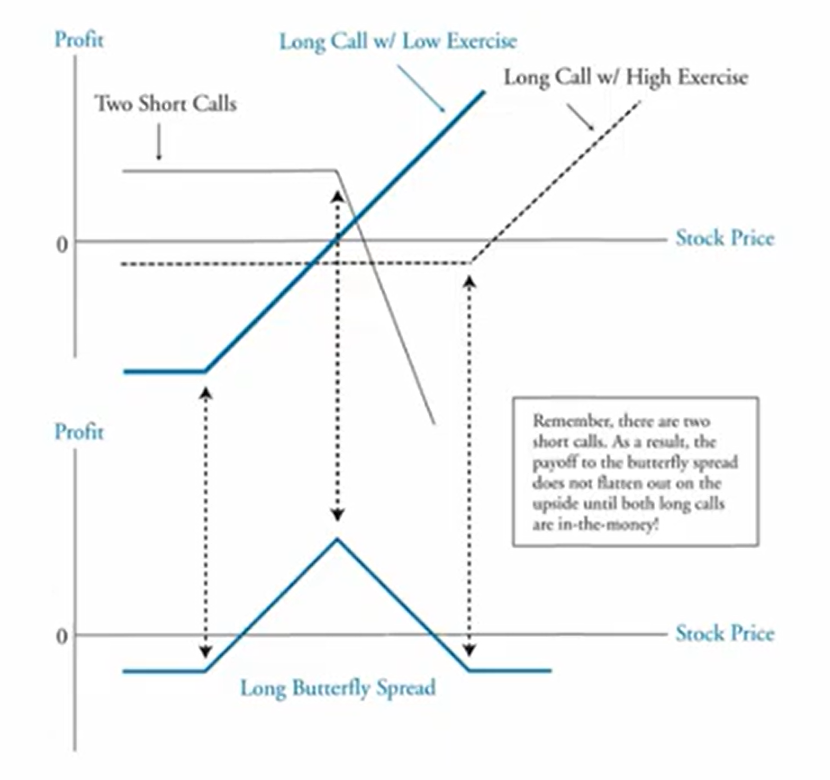
\includegraphics[width=0.4\textwidth]{long butterfly spread.png}
    \centering    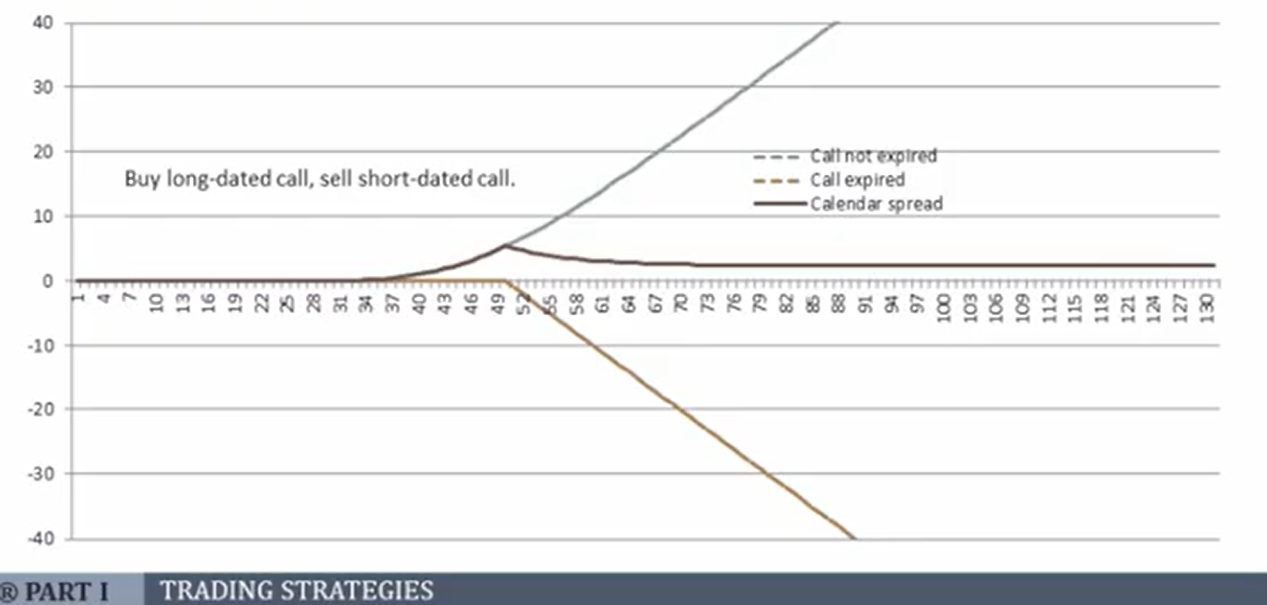
\includegraphics[width=0.4\textwidth]{calendar spread.png}
\end{wrapfigure}


 \textbf{Short Butterfly call spread:}
 \begin{itemize}
 \item Продать: call опцион с \textbf{меньшей} strike ценой.\\
Купить:2  call опцион с \textbf{средней} strike ценой.\\Продать: call опцион с \textbf{большей} strike ценой.
\item Предположение: высокая волатильность.
\item Максимальная прибыль: $(X_H - X_L) + (-C_L +2C_M -C_H) $
\item Максимальный убыток:$ -C_L +2C_M -C_H $
\item Цена перелома: $ X_L - (-C_L + 2C_M - C_H) $
\end{itemize}


 \textbf{Long Butterfly call spread:}
 \begin{itemize}
 \item Купить: call опцион с \textbf{меньшой} strike ценой.\\
Продать:2  call опцион с \textbf{средней} strike ценой.\\Купить: call опцион с \textbf{большей} strike ценой.
\item Предположение: низкая волатильность.
\item Максимальная прибыль: $(X_H - X_L) + (-C_L +2C_M -C_H) $
\item Максимальный убыток:$ -C_L +2C_M -C_H $
\item Цена перелома: $ X_L - (-C_L + 2C_M - C_H) $
\end{itemize}

\textbf{Calendar spread:}
 \begin{itemize}
 \item Два опциона.
\item Одинаковая strike цена.
\item Разное время экспирации.
\end{itemize}
\textbf{Directions:}
 \begin{itemize}
 \item Direct calendar spread - купить long-dated, продать short-dated (предполагаем низкую волатильность).
\item Reverse calendar spread - купить short-dated, продать long-dated (предполагаем высокую волатильность) 
\end{itemize}

\textbf{Категории:}
 \begin{itemize}
 \raggedright
\item Нейтральная: strike цена около текущей рыночной стоимости.
\item Bearish: strike цена ниже текущей рыночной стоимости.
\item Bullish: strike цена выше текущей рыночной стоимости.
\end{itemize}
\newpage
 \section{Использование и выплата в различных комбинированных стратегиях}\\
 
 \begin{wrapfigure}{}{0.4\textwidth}
    \centering    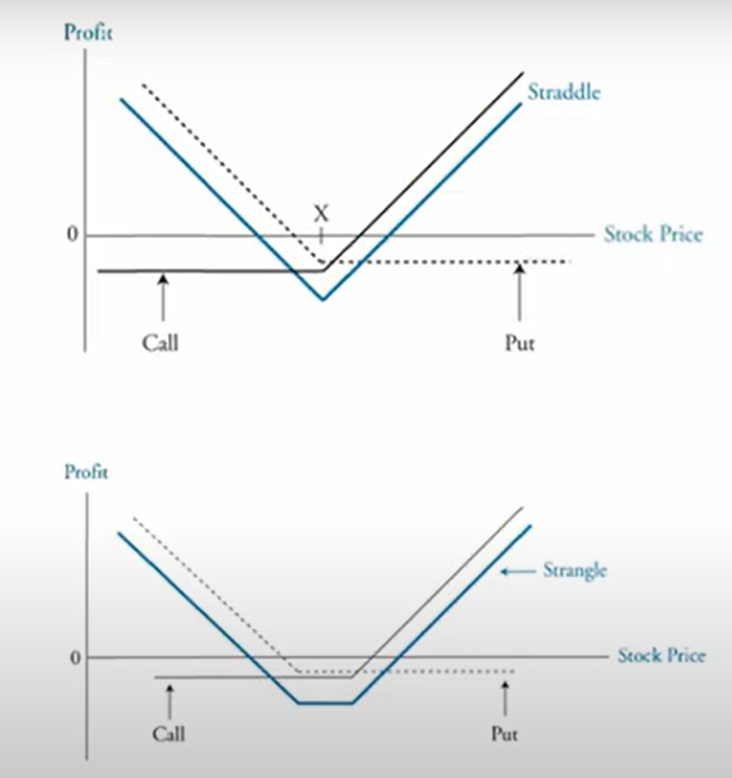
\includegraphics[width=0.4\textwidth]{straddle n strangle.png}
\end{wrapfigure}

 \textbf{Long straddle:}
 \begin{itemize}
 \item Купить: call опцион.\\
Купить: put опцион с \textbf{такой же} strike ценой.
\item Предположение: волатильность вырастет.
\item Максимальная прибыль: неограничена.
\item Максимальный убыток: $ -P - C $
\item Цена перелома: $ X - (-P - C) $ и $ -P - C $
\end{itemize}

\textbf{Long strangle:}
 \begin{itemize}
 \item Купить: call опцион с \textbf{большей} strike ценой..\\
Купить: put опцион с \textbf{меньшей} strike ценой.
\item Предположение: волатильность вырастет.
\item Максимальная прибыль: неограничена.
\item Максимальный убыток: $ -P - C $
\item Цена перелома: $ X_H - (-P - C) $ и $ X_L + ( -P - C) $
\end{itemize}


\begin{wrapfigure}{}{0.4\textwidth}
    \centering    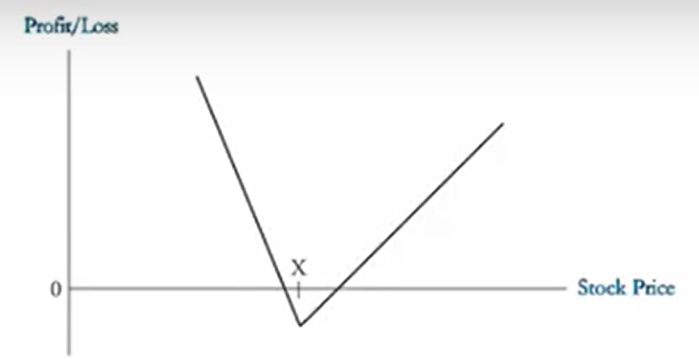
\includegraphics[width=0.4\textwidth]{strip strap.png}
\end{wrapfigure}

 \textbf{Long strip:}
 \begin{itemize}
 \item Купить: call опцион.\\
Купить: 2 put опциона с \textbf{такой же} strike ценой.
\item Предположение: цена будет двигаться, но движение вниз более вероятно.
\item Максимальная прибыль: неограничена.
\item Максимальный убыток: $ -2P - C $
\end{itemize}

 \textbf{Long strap:}
 \begin{itemize}
 \item Купить: 2 call опциона.\\
Купить: put опцион с \textbf{такой же} strike ценой.
\item Предположение: цена будет двигаться, но движение вверх более вероятно.
\item Максимальная прибыль: неограничена.
\item Максимальный убыток: $ -P - 2C $
\end{itemize}

 \textbf{Diagonal spread:}
 \begin{itemize}
 \item 2 опциона.
\item Разная strike цена.
\item Разное время экспирации.
\end{itemize}


\begin{wrapfigure}{}{0.4\textwidth}
    \centering    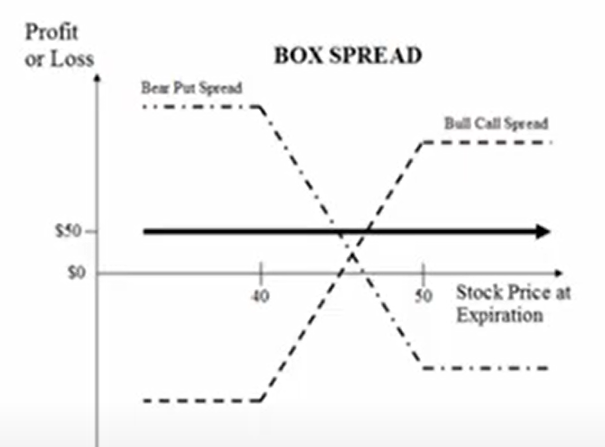
\includegraphics[width=0.4\textwidth]{box.png}
\end{wrapfigure}

 \textbf{Box spread:}
 \begin{itemize}
 \item Bull call spread + bear put spread.
\item Фиксированная положительная выплата.
\item Только европейские опционы.
\item Используют для арбитража.
\end{itemize}

\end{document}
